\documentclass[format=sigconf]{acmart}
\acmConference[ICONS 2020]{International Conference on Neuromorphic Systems}{July 2020}{Chicago, Illinois}
\keywords{Equilibrium Propagation, vanishing gradient problem, small-world}

%\usepackage{cite}
\usepackage{natbib}
\usepackage{graphicx}
\usepackage{bm}
\usepackage{amsmath}
%\usepackage{amssymb}
\usepackage{subcaption}
\usepackage{mathtools}
\usepackage[titletoc]{appendix}
\usepackage[ruled,vlined]{algorithm2e}
\usepackage{hyperref}

\newcommand{\mtx}[1]{\bm{#1}}
\newcommand{\rms}[1]{<{#1}>}
\newcommand{\npar}{\\\indent}

\title{Layer-skipping connections facilitate training of layered networks using equilibrium propagation.}
\author{Jimmy Gammell}
\author{Adam McCaughan}

\begin{document}

\begin{abstract}

Equilibrium propagation is a learning framework for energy-based networks that can be implemented by neurons that perform only one type of computation in the prediction and correction phases of training, and that computes parameter corrections for a given neuron using only the activation values of directly-connected neurons. This makes it an appealing candidate for implementation in neuromorphic analog hardware, and marks a step forward in the search for a biologically-plausible implementation of deep learning. However, in previous implementations of equilibrium propagation, layered networks of any depth suffered from a vanishing gradient problem that has not yet been solved in a simple or biologically-plausible way. In this paper, we demonstrate that modifying the layered topology by adding random layer-skipping connections in a manner inspired by small-world networks can counteract the vanishing gradient problem to significantly facilitate training. This approach could be conveniently implemented in neuromorphic analog hardware and is biologically-plausible.

\end{abstract}

\maketitle

\section{Introduction}

The equilibrium propagation learning framework \cite{scellier17} is a method for training a class of energy-based networks, the prototype for which is the continuous Hopfield network \cite{hopfield1984}. It is appealing as a framework that could be implemented in neuromorphic analog hardware because unlike in backpropagation, neurons are required to perform only one type of computation in the prediction of correction phases of training, and the parameters of a neuron can be updated using only the activations of neurons to which it is directly connected - there is no need for feedback paths through which to transmit information about the parameters and states of neurons across the entire network. Backpropagation is not biologically plausible, and a major reason is that credit assignment to a given neuron requires precise knowledge of the nonlinearities and derivatives of all neurons in the feedforward path between that neuron and the output\cite{bengio2015}; equilibrium propagation avoids this issue. Another major reason is that it is implausible for the forward and backwards propagation phases to use different computations requiring different computational circuits \cite{scellier17}; equilibrium propagation also avoids this issue.
\npar
It has been demonstrated \cite{scellier17} that a continuous Hopfield network with a basic multilayer topology can be trained on MNIST \cite{mnist1998} through the equilibrium propagation framework. However, previous implementations encountered a vanishing gradient problem that significantly impedes training of networks with several hidden layers. Given that network depth is critical for performance on difficult datasets \cite{simonyan2014, srivastava2015tvdn}, and that convergence to a low error rate on MNIST is a low bar for a network to meet, this is a nontrivial issue. It has been demonstrated \cite{scellier17} that the problem can be solved by using a unique learning rate for parameters at different depths in the network, with deeper parameters trained with larger learning rates to counteract gradient attenuation with depth. This approach is unappealing because (1) it introduces additional hyperparameters that must be tuned, (2) it would be inconvenient to implement and tune unique learning rates in analog hardware, and (3) it seems unlikely that it is biologically plausible.
\npar
The purpose of this paper is to introduce a modification to the basic multilayer topology that can counteract the vanishing gradient problem in the context of energy-based networks trained using equilibrium propagation. We fully connect a network's layers, then replace a small portion of its connections with random layer-skipping connections, in a manner inspired by small-world networks \cite{watts98}. We achieve 0\% training error and under 2.5\% test error on MNIST using a network with 3 hidden layers and no regularization term in its cost function. These error rates are competitive (**this may be too generous) in the context of similar biologically-motivated networks \cite{bartunov2018} and are the same as those achieved by a basic multilayer network with 3 hidden layers in the original paper using a basic topology and unique learning rates \cite{scellier17}, albiet they are achieved after around 25\% more epochs. Our method adds only one additional hyperparameter
\footnote{In our current implementation we tune the initial weights for added connections independently of those of preexisting connections. We have found that networks are not very sensitive to these initializations and that performance is good if they are in the same ballpark as initializations of preexisting connections (though we have no mathematical justification for this); thus, we do not consider this to be an additional hyperparameter.}
 - the number of connections to randomly replace - and could be implemented with relative ease in analog hardware. Layer-skipping connections seem biologically-plausible, and small-world networks have been documented in biological brains \cite{bullmore2009}. Similar techniques have been used with some success in convolutional \cite{he2015, srivastava2015} and basic multilayer feedforward \cite{xiaohu2011, krishnan2019} networks with varying degrees of success. Our findings in this paper show that layer-skipping connections are effective enough to be appealing in contexts where simplicity and biological plausibility are important, but would likely not make sense for use in a digital implementation of equilibrium propagation where performance is a primary consideration.


\section{Background and Theory}

\subsection{Equilibrium propagation}
\label{sec:eqp_formulation}

Equilibrium propagation \cite{scellier17} is a learning framework for energy-based networks that trains their parameters by approximating gradient descent on some arbitrary cost function. It is applicable to any network with dynamics characterized by evolution to a fixed point of an associated energy function; in this and in the original paper, it is implemented on a continuous Hopfield network \cite{hopfield1984}. For a variety of reasons outlined in \cite{bengio2015}, backpropagation is not biologically-plausible. One of the major reasons is that to correct the parameters of a given neuron, backpropagation requires precise information about the activations and nonlinearities of all neurons in the corresponding feedforward path, and no mechanism capable of delivering this information has been observed in biological brains. Equilibrium propagation avoids this problem by approximating the gradient of an arbitrary cost function with respect to a neuron's parameters using only the activations of neurons to which it directly connects. Another major reason backpropagation is not biologically-plausible is that it requires neurons to perform distinct computations (implemented using distinct circuitry) in the forward and backward propagation phases of training, and no evidence suggests that biological neurons perform distinct computations during distinct phases of learning. In contrast, equilibrium propagation requires only one behavior of neurons in both the prediction (free) and correction (weakly-clamped) phases of training: that over time they adjust their activation functions to perform gradient descent on an associated energy function (though this is still biologically-implausible because it requires two distinct phases of training). In addition to enhancing its biological plausibility, these traits also make equilibrium propagation appealing as a framework to implement on neuromorphic analog hardware because they would limit the complexity required of neurons and the amount of infrastructure needed to operate and train them.

\subsubsection{Implementation in a continuous Hopfield network}

Here we summarize the dynamics of a continuous Hopfield network trained using equilibrium propagation; a more-thorough and more-general treatment, on which this summary is based, is given in the original paper \cite{scellier17}.
\npar
Consider an arbitrary network with two subsets of its neurons designated as an input and output layer. Let $\mtx{x}$, $\mtx{h}$, and $\mtx{y}$ denote, respectively, vectors containing the activations of its input, hidden and output layers, $\mtx{s}=\{\mtx{h},\mtx{y}\}$ denote its state and $\mtx{u}=\{\mtx{x}, \mtx{h},\mtx{y}\}$ denote its full set of neurons. Let $\mtx{W}$ and $\mtx{b}$ denote its weights and biases and $\rho$ denote the activation function of a neuron; here and in the original paper it is a hardened sigmoid function 
\begin{equation}
\label{eqn:hardened_sigmoid}
\rho(x)=\begin{cases}0&x<0 \\ x&0\leq x \leq 1 \\ 1&x>1\end{cases}
\end{equation} with
\begin{equation}
\rho'(x):=\begin{cases}0&x<0\\1&0\leq x \leq 1\\0&x>1\end{cases}
\end{equation}
where the derivative is defined to be 1 at endpoints of its support to avoid saturation. Let $\mtx{x}_d$ and $\mtx{y}_d$ denote the input and target output from a training dataset during a given batch.
\npar
A prediction $\mtx{y}$ of $\mtx{y}_d$ is generated by clamping $\mtx{x}$ to $\mtx{x}_d$, then evolving to a local minimum of an energy function
\begin{equation}
E(\mtx{u})=\frac{1}{2}\sum_iu_i^2-\frac{1}{2}\sum_{i\neq j}W_{ij}\rho(u_i)\rho(u_j)-\sum_ib_i\rho(u_i).
\end{equation}
This initial prediction-generating evolution is denoted the free phase. Consider some cost function $C(\mtx{u}, \mtx{W}, \mtx{b}, \mtx{y}_d)$; in this and in the original paper it is a quadratic error function
\begin{equation}
\label{eqn:cost}
C(\mtx{y},\mtx{y}_d)=\frac{1}{2}||\mtx{y}-\mtx{y}_d||_2^2,
\end{equation}
but the algorithm is applicable to an arbitrary cost function - for example, one including a regularization term. After the free phase, the network is then evolved to a local minimum of a total energy function
\begin{equation}
F(\mtx{u},\mtx{y}_d, \beta)=E(\mtx{u})+\beta C(\mtx{y},\mtx{y}_{target})
\end{equation}
where $\beta$, called the clamping factor, is a small constant. Note that $E(\mtx{u})=F(\mtx{u},\mtx{y}_d,0)$; therefore, the free phase can (and, henceforth, will) be interpreted as evolution to equilibrium on $F(\mtx{u},\mtx{y}_d,0)$. This second phase is denoted the weakly-clamped phase, and can be interpreted as first nudging the output neurons in the direction of the target output, then allowing remaining neurons to adjust towards a configuration that would have predicted the more-correct nudged output (though it is unclear that this interpretation would hold if a regularization term were added to the cost function). The network evolves to equilibrium by performing gradient descent on $F$ through the equation of motion
\begin{equation}
\label{eqn:dynamics}
\frac{d\mtx{s}}{dt}=-\frac{\partial F}{\partial \mtx{s}}.
\end{equation}
The states of the network after the free and weakly-clamped phases are used to compute correction terms so must be saved; after evolution on some set of training data we will denote these states, respectively, $\mtx{s}^0$ and $\mtx{s}^{\beta}$. The process for training over a set of data is as follows:
\begin{enumerate}
\item Perform the free-phase evolution; evolve to equilibrium on the energy function $F(\mtx{u}, \mtx{y}_d, 0)$ by updating $\mtx{s}$ according to equation \ref{eqn:dynamics}. Record the equilibrium state $\mtx{s}^0$.
\item Perform the weakly-clamped evolution; evolve for a short amount of time towards equilibrium on the energy function $F(\mtx{u},\mtx{y}_d,\beta)$, again according to equation \ref{eqn:dynamics}, using $\mtx{s}^0$ as a starting point. Record the equilibrium state $\mtx{s}^{\beta}$.
\item Compute the correction to each weight in the network using the function 
\begin{equation}
\label{eqn:weight_correction}
\Delta W_{ij}=\alpha \frac{1}{\beta}(\rho(u_i^\beta)\rho(u_j^\beta)-\rho(u_i^0)\rho(u_j^0))
\end{equation}
where $\alpha$, the learning rate, is a positive constant. Adjust the weights using $W_{ij}:=W_{ij}+\Delta W_{ij}$.
\item Compute the correction to each bias in the network using the function
\begin{equation}
\Delta b_i=\alpha \frac{1}{\beta}(\rho(u_i^{\beta})-\rho(u_i^0))
\end{equation}
and adjust the biases using $b_i:=b_i+\Delta b_i$.
\end{enumerate}
Note that the correction to a weight depends only on the activations of neurons it directly affects, and the correction to a bias depends only on the activation of the neuron it directly affects. This is in contrast to backpropagation, where to correct a weight or bias $l$ layers from the output it would be necessary to know the activations, derivatives and weights of all neurons between $0$ and $l-1$ layers from the output.

\subsubsection{Approximation of equation of motion}

In analog hardware, the dynamics described by equation \ref{eqn:dynamics} could be implemented efficiently using leaky integrator neurons. On digital hardware, however, it is necessary to discretize and approximate the differential equation of motion; we now describe the approximation used here and in the original paper. Let $\mtx{s}[n]$ denote the state of the network after $n$ iterations of the approximation, $N$ denote the total number of iterations and $\epsilon$ the size of each iteration. $\mtx{s}[0]$ is the initial state of the network; this may be random or, as in this and the original paper, zero.  Let 
 \begin{equation}
 s_i[n]=s_i[n-1]-\epsilon \frac{\partial F}{\partial s_i}(\mtx{u},\mtx{y}_d,\beta),\;n=1,\hdots,N.
 \end{equation}
 Then the state of the network after time $\tau=\epsilon N$ is given by
\begin{equation}
\int_0^\tau\frac{d\mtx{s}}{dt}dt\approx \mtx{s}[N].
\end{equation}
 We denote the number of iterations in the free and weakly-clamped phases $N_{free}$ and $N_{weakly-clamped}$, respectively. It is only necessary to run the weakly-clamped phase long enough to observe the initial direction in which the network evolves and to allow the perturbation of the output to influence all layers in the network, so typically for a network with $L$ layers $N_{free}>>N_{weakly-clamped}>L$.
 
\subsubsection{Applicable methods for enhanced biological-plausibility}

A major reason backpropagation is not biologically-plausible is that it implies a set of feedback connections with weights and destinations identical to the feedforward connections; this is also an issue in equilibrium propagation. However, recent work \cite{lillicrap2014} has shown that networks can still train if feedback weights are initialized randomly instead of symmetrically with feedforward connections, and that with training their weights will become similar to forward weights. These findings could be applied to an energy-based network trained using equilibrium propagation.
\npar
Biological neurons are known to communicate through spikes with binary values, suggesting that a spike timing based activation function for neurons is more biologically-plausible than popular functions. It has been shown \cite{oconnor2018} that an energy-based network with a spike timing-based activation function can be trained using equilibrium propagation.
\npar
The method presented in this paper allows networks with multiple layers to train effectively through a biologically-plausible tweak to their topology. Layer-skipping connections have been documented in biological brains \cite{bullmore2009}.

\subsection{Vanishing gradient problem}
\label{sec:vangrad}

It has been observed \cite{scellier17} that energy-based networks with a layered topology trained using equilibrium propagation suffer from a vanishing gradient problem: the magnitude of the weight correction matrix to weights between a pair of layers attenuates exponentially with the number of layers between that pair and the output layer. This problem is familiar in the context of conventional networks trained through backpropagation, where if the magnitude of the correction matrix to weights connecting the output layer to the last hidden layer is $\Delta W$ and if the expected magnitude of the derivative of neurons' activation function is $\alpha<1$, then the magnitude of the correction matrix to weights connecting layers $l$ and $l-1$ from the output is expected to be $\alpha^l\Delta W$. In conventional networks, the vanishing gradient problem can be effectively addressed by initializing weights to make activation variances and backpropagated gradient variances approximately uniform with respect to depth as described in \cite{glorot2010} and by using activation functions with unity derivatives (**find reference), such as rectified linear units $\rho(x)=\text{Max}\{0, x\}$ or hardened sigmoids (equation \ref{eqn:hardened_sigmoid}).
\npar
Neither of these approaches are effective at solving the vanishing gradient problem in the context of equilibrium propagation. In the context of energy-based networks the situation is more-complicated because there is no straightforward causal relationship between the activations of two given neurons; instead, neurons evolve as a system. The fact that conventional approaches are ineffective suggests that the cause of the problem is different than in conventional networks.
\npar
The vanishing gradient problem causes deep networks to train very slowly, which is obviously undesirable. It also causes the magnitudes of corrections to weights between pairs of layers to differ by many orders of magnitude, which would be problematic in an analog implementation of the framework using neurons with limited numerical precision.
\npar
In the original paper the vanishing gradient problem was solved by using unique learning rates for each layer, chosen to make the magnitudes of corrections to neurons' parameters uniform regardless of depth in the network. While this method was effective, it is unappealing because it seems unlikely to take place in a biological brain, it would add complexity to an analog implementation of the framework, and it introduces more hyperparameters that must be tuned to train a network. Our topology solves the problem without these unappealing characteristics.

\subsubsection{Contribution by approximation of equation of motion}

One factor that probably contributes to the vanishing gradient problem is that when the output layer of neurons is perturbed at the beginning of the weakly-clamped phase, it takes an additional iteration of the approximation of equation \ref{eqn:dynamics} for the perturbation to influence the last hidden layer, then an additional iteration for the second-to-last hidden layer, and so on. We do not believe this factor to be a significant contributor to the vanishing gradient problem because increasing $N_{weakly-clamped}$ does not significantly affect network performance. This is supported by the following rough theoretical formulation:
\npar
Assume that a typical neuron in the network changes by a small constant amount $\delta$ after each iteration of equation \ref{eqn:dynamics} (this is reasonable because we run only the early stages of evolution to the weakly-clamped equilibrium), and assume that the typical neuron is in state $s_0$ at the end of the free phase. After $N$ iterations, a neuron in the output layer will have changed by $N\delta$ and one in a deep layer $l$ layers from the output will have changed by $(N-l)\delta$. Assume further that $s_0$ is in the middle of the support of $\rho'$ where $\rho$ is the hardened sigmoid function from equation \ref{eqn:hardened_sigmoid}, so that we can replace $\rho(x)$ by $x$. Then it follows from equation \ref{eqn:weight_correction} that a typical neuron in the output layer will be corrected by 
\begin{equation}
\Delta w^\text{output}=\frac{\alpha}{\beta}((N\delta + s_0)((N-1)\delta + s_0)-s_0^2)\approx \frac{\alpha}{\beta}(N^2\delta^2+2s_0N\delta)
\end{equation}
and similarly a typical neuron from the deep layer will be corrected by 
\begin{equation}
\Delta w^l\approx \frac{\alpha}{\beta}((N-l)^2\delta^2+2s_0(N-l)\delta)
\end{equation}
(where we have approximated $N\approx N-1$ and $N-l+1\approx N-l$), so the ratio of these corrections will be
\begin{equation}
\frac{\Delta w^l}{\Delta w^{\text{output}}}\approx \frac{(N-l)^2\delta^2-2s_0(N-l)\delta}{N^2\delta^2+2s_0N\delta}=\frac{N-l}{N}\frac{(N-l)\delta+2s_0}{N\delta+2s_0}\approx 1-\frac{l}{N}
\end{equation}
(where we have approximated $\frac{(N-l)\delta +2s_0}{N\delta+2s_0}\approx 1$). We have observed that
\begin{equation}
\frac{\Delta w^l}{\Delta w^{\text{output}}}\sim 4^{-l},
\end{equation}
for the type of networks we tested, so it seems unlikely that this phenomenon is a primary cause of the vanishing gradient problem.

\subsection{Small-world networks}
\label{sec:sw_background}

Our topology was inspired by small-world graph topology as described in \cite{watts98}. We have observed that energy-based networks with layered topology experience exponential attenuation of the gradient of a given parameter as its depth in the network increases, so it seems reasonable to expect that the vanishing gradient problem can be reduced by decreasing the number of connections needed to move between a given neuron and the output layer. Small-world topology offers a way to do this while largely preserving clustering between neurons within the same layer. It is also a topology that has been observed in biological brains \cite{bullmore2009}. Essentially, a layered network with fully-connected layers can be viewed as a network with a large typical path length between pairs of neurons and a large amount of clustering between nearby neurons. By randomly replacing a small proportion of its connections, its typical path length can be greatly reduced without significantly affecting its clustering.
\subsubsection{Small-world metrics}
The small-worldness of a network is typically characterized by two metrics: a characteristic path length $L$ and a clustering coefficient $C$. A graph is small-world if $L$ is small relative to the $L$ of a random network with the same number of vertices and edges and $C$ is not substantially smaller than the $C$ of that random network. The characteristic path length is the minimal number of edges in a path joining a pair of vertices, averaged over all pairs of vertices in the network. Specifically, for a graph with $N$ vertices where $l(v_i,v_j)$ denotes the smallest number of edges needed to connect vertex $v_i$ to vertex $v_j$, 
\begin{equation}
\label{eqn:charpathlength}
L=\frac{1}{N(N-1)}\sum_{i=1}^{N}\sum_{\substack{j=1\\j\neq i}}^{N}l(v_i,v_j).
\end{equation}
The neighborhood of a vertex is the set of vertices with which it shares an edge. The clustering coefficient is the proportion of pairs of vertices in the neighborhood of a given vertex that share an edge, averaged over all vertices in the network. Specifically, for a graph with $N$ vertices, if $\text{N}(v_i)$ denotes the neighborhood of vertex $v_i$ and $c(v_j,v_k)=\begin{cases}1 & v_k\in\text{N}(v_j)\\0 & \text{else}\end{cases}$,
\begin{equation}
\label{eqn:clustcoeff}
C=\frac{1}{N}\sum_{i=1}^{N}\frac{1}{|\text{N}(v_i)|}\sum_{\substack{v_j\in \text{N}(v_i)\\v_k\in\text{N}(v_i)\\j\neq k}}c(v_j,v_k)
\end{equation}
\npar
An algorithm was introduced in \cite{watts98} to convert a regimented graph into a small-world graph
\footnote{Our algorithm is actually slightly different: instead of replacing each edge with probability $p$, at each step we randomly select $n$ of the existing edges and replace them with random edges. For a network with $N$ edges our algorithm is on average equivalent to the one from \cite{watts98} with $p=1-(\frac{N-1}{N})^n$. For ease of comparison with other work and to contextualize how many edges have been replaced, we will henceforth describe networks using our topology in terms of $p$ and not $n$.}.
 For each existing edge in the network, with probability $p$: randomly pick a pair of vertices that do not share an edge. Add an edge between these vertices, and remove the existing edge. As $p\approx 0$ is increased, $L$ initially decreases much more quickly than $C$. $p$ is typically chosen so that $L$ has decreased substantially and $C$ has just begun to decrease.
\subsubsection{Small-world metrics have little correlation with network performance}
Contrary to our expectations, we found that a network's performance does not track closely with its clustering coefficient or characteristic path length, and that good performance is achieved when the above algorithm is executed with $p\approx 8\%$, which is substantially higher than the value of $p$ that would make its topology small-world. We believe that our qualitative arguments about the merits of a small-world network are sound, but that the characteristic path length and clustering coefficient are poor predictors of the performance of a deep neural network. The characteristic path length does not take into account the number of low-attenuation paths a neuron can take to the output layer, but clearly this is an important factor, since a neuron's behavior is dictated by an affine combination of all its inputs. While it is important for a network to retain its layered nature in order to generalize well, the clustering coefficient does not appear to be a good metric for this - e.g. a layered network without intralayer connections has a small clustering coefficient because the neighbors of a given neuron are not connected to one-another.
\npar
There are several factors other than path length that we expect have an effect on performance as the value of $p$ is changed, and it is possible that they disguise relationships with the small-world metrics. It has been shown \cite{he2015} that in deep convolutional networks, performance can be improved by using layer-skipping connections to create a linear transformation (e.g. an identity mapping) in parallel with sets of nonlinear layers to reframe their task as learning the residual of the output of earlier layers; in our implementation layer-skipping connections form a linear transformation of earlier layers, and this fact may improve performance even though only some of the dimensions of the deeper layers are transferred. We discussed in section \ref{sec:vangrad} that deep layers experience less evolution than shallow layers during the weakly-clamped phase; since layer-skipping connections allow deeper layers to begin to evolve sooner, we expect that they reduce this effect. As connections are replaced, a network looks less layered and more like a sparsely-connected single-layer network, so we expect that there is a tradeoff between the rate at which a network trains and its ability to generalize. In this paper our topology did not deteriorate test error relative to the original layered network, but it is highly possible that a network on a harder dataset (e.g. CIFAR or ImageNet) or with a higher value of $p$ would see deterioration as its topology deviates from a layered topology.

\subsection{Nonlinearities learning residuals}
\label{sec:residuals}

It has been shown \cite{he2015, ioffe2015} that the performance of very-deep convolutional networks can be improved by using layer-skipping connections to create an identity mapping or other dimension-preserving linear transformation in parallel with groups of layers constituting nonlinear transformations. For a network without layer-skipping connections on a dataset $\{\mtx{x}_d,f(\mtx{x}_d)\}$, consider a group of layers. If the output of preceding layers is $g(\mtx{x}_d)$, the task of those layers is to learn $f(g^{-1}(\mtx{x}))\approx \mtx{x}$ since the preceding layers have presumably trained to approximate $f$. Therefore, this task can be made easier by adding an identity mapping or linear transformation in parallel with the group of layers to reframe their task as finding the residual of the preceding layers $f(g^{-1}(\mtx{x}))-\mtx{x}$, since it is easier to drive the output of a group of neurons towards zero than it is to make it approximate an arbitrary transformation.
\npar
Since layer-skipping connections constitute a linear transformation of a deep layer into a shallower layer, the above is a possible contributor to the effectiveness of layer-skipping connections; the MNIST dataset has a significant linear component, and of the hardened sigmoid activation function does a poor job of representing the underlying function, the network's effectiveness may be improved by skipping some of its hardened-sigmoid-based transformations using linear layer-skipping connections.


\section{Related work}

Much research has been done in pursuit of a biologically-plausible deep learning algorithm. \cite{lee2015}, \cite{xie2003} and \cite{pineda1987} are other algorithms that address the weight transport problem. \cite{lillicrap2014} addresses the need for symmetric feedback weights, a problem not addressed by equilibrium propagation. \cite{oconnor2018} implements equilibrium propagation using spiking neurons like are present in a biological brain. \cite{bengio2015} and \cite{???} discuss the criteria such an algorithm would need to satisfy. \cite{bartunov2018} surveys promising biologically-motivated algorithms and evaluates their effectiveness on hard algorithms.
\npar
\cite{shainline2019}, \cite{davies2018} and \cite{nahmias2013} discuss neuromorphic architecture that could potentially implement equilibrium propagation as an analog computer.
\npar
Layer-skipping connections have been explored in other contexts. \cite{he2015} and \cite{srivastava2015} use layer-skipping connections as a linear transformation in parallel with nonlinear layers to great effect in very-deep convolutional networks. \cite{xiaohu2011} and \cite{krishnan2019} use a small-world topology in conventional multilayer feedforward networks.
\npar
The vanishing gradient problem was a big obstacle to the training of conventional deep networks through backpropagation, and \cite{ioffe2015}, \cite{glorot2010} and \cite{???} provide effective means for solving it in that context.



\section{Implementation}

\begin{figure}
  \centering
  \begin{subfigure}[t]{.48\textwidth}
    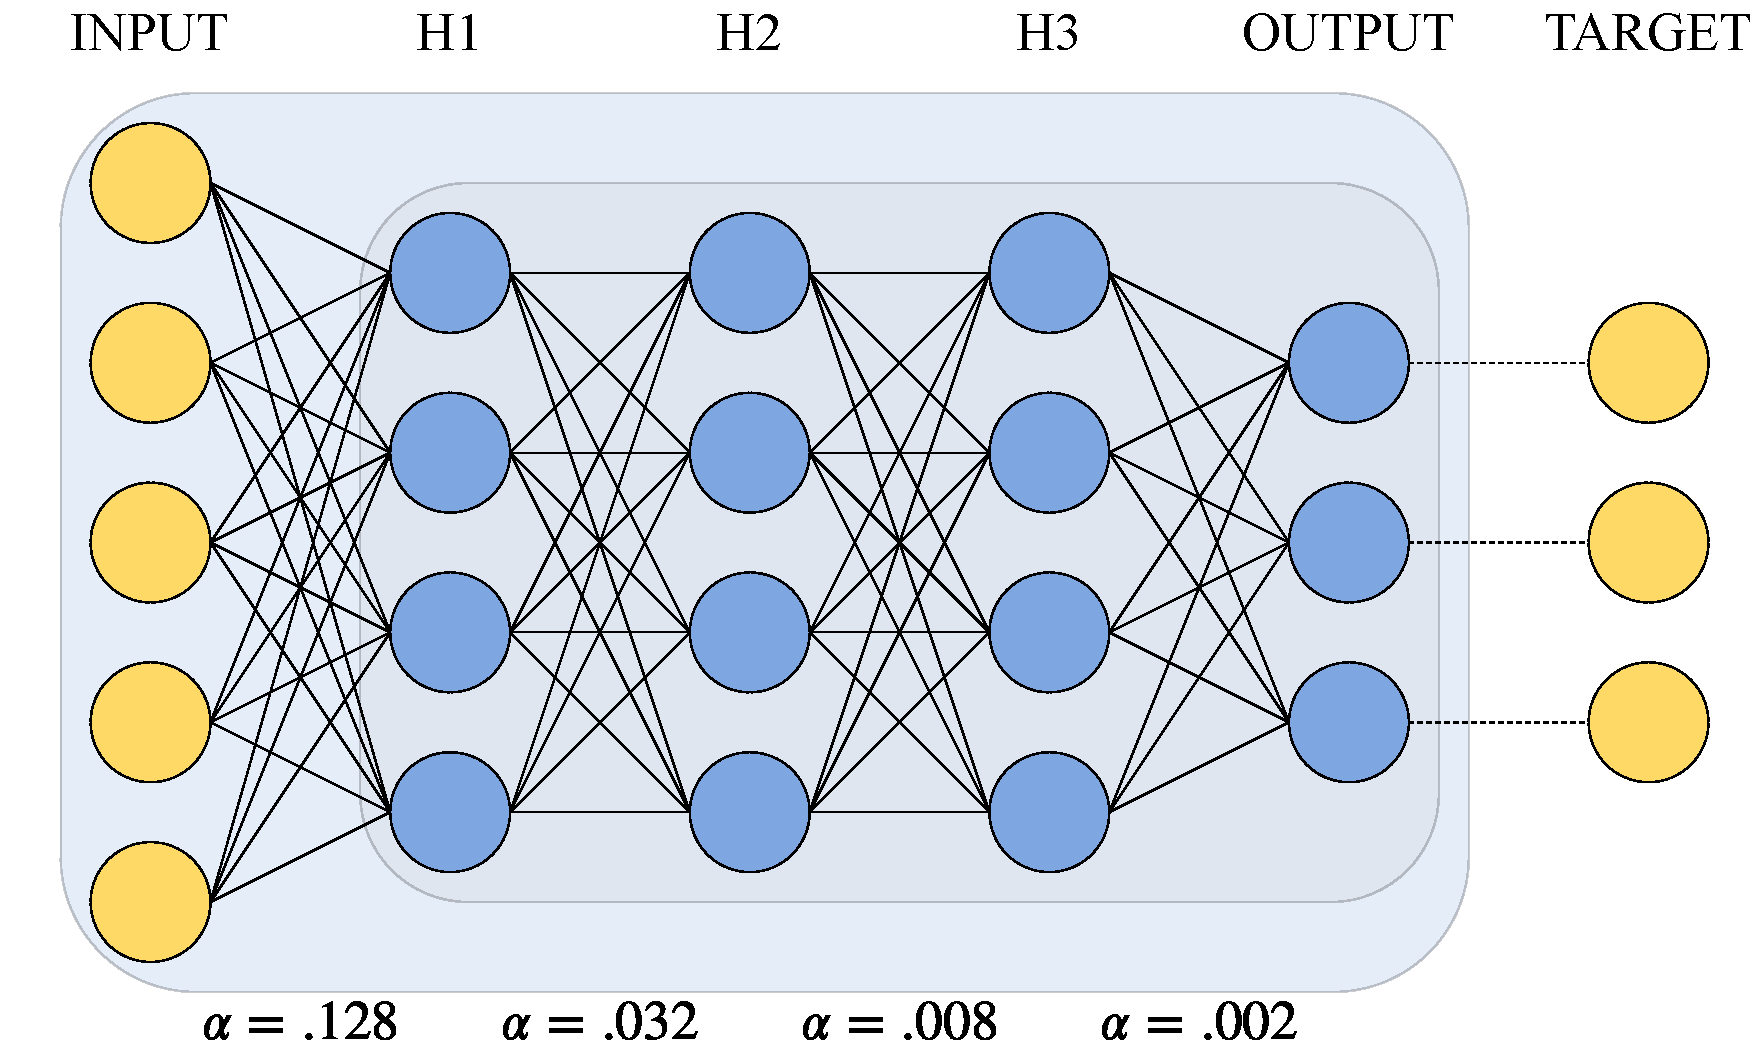
\includegraphics[width=.9\textwidth]{figures/basic_topology_illustration.pdf}
    \caption{Topology of the basic multilayer network tested in \cite{scellier17}. All pairs of neurons in adjacent layers are connected, and there are no additional connections. The learning rate for weights is reduced by a factor of 4 each time distance from the output decreases by one layer, to compensate for the vanishing gradient problem (section \ref{sec:vangrad}).}
    \label{fig:top_basic}
  \end{subfigure}
  \hfill
  \begin{subfigure}[t]{.48\textwidth}
    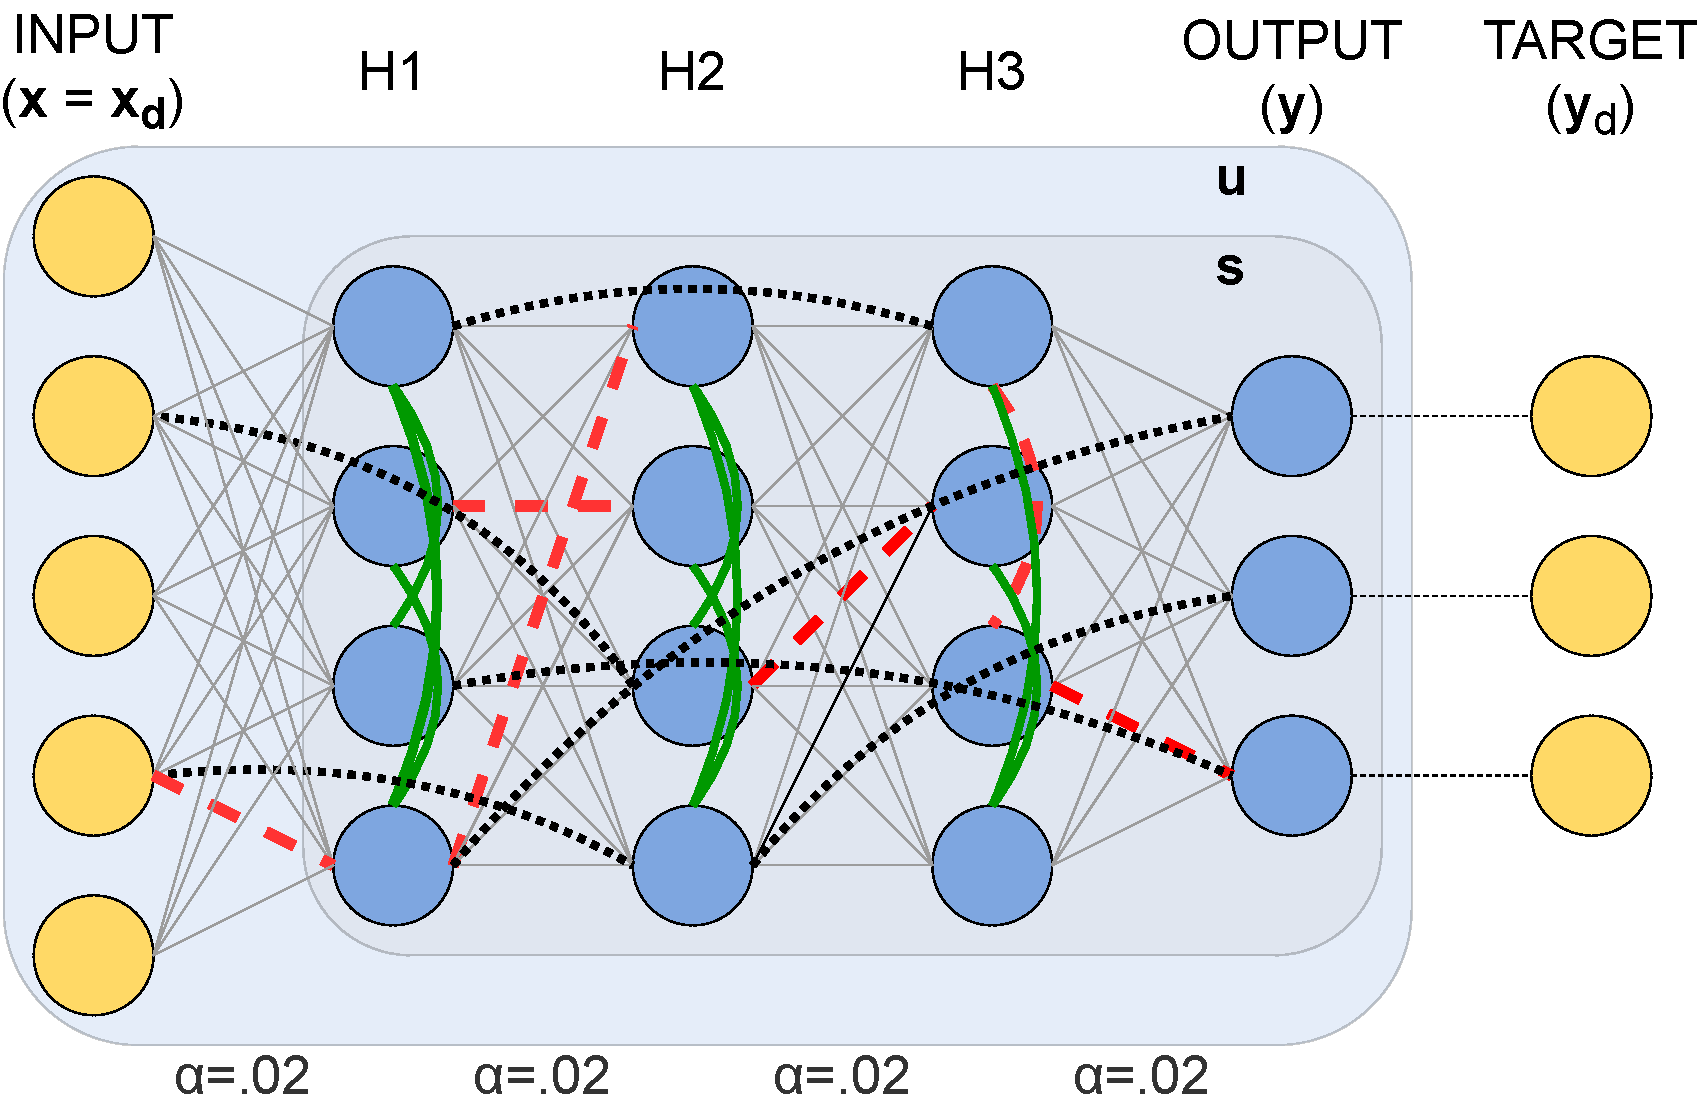
\includegraphics[width=.9\textwidth]{figures/topology_changes_illustration.pdf}
    \caption{Changes we have made to the basic topology to compensate for the vanishing gradient problem (section \ref{sec:vangrad}) while using a single learning rate for all weights. Red dotted lines denote connections that have been removed and blue lines denote their replacements. Green lines denote added connections within layers (these are also candidates for replacement). In this illustration layers have been made fully connected, and each connection has then been replaced by a random layer-skipping connection with probability $p\approx 8\%$.}
    \label{fig:top_sw}
  \end{subfigure}
  \caption{}
  \label{fig:topology_illus}
\end{figure}

We implemented
\footnote{\url{https://github.com/jgammell/Equilibrium_Propagation_mobile.git}}
 the equilibrium propagation learning framework \cite{scellier17} using the Pytorch library \cite{pytorch}, and verified that we could recreate the experiments run in \cite{scellier17}. We follow the procedure described in section \ref{sec:eqp_formulation}; we use a hardened sigmoid activation function (equation \ref{eqn:hardened_sigmoid}) and a squared-error cost function with no regularization term (equation \ref{eqn:cost}). Testing was done on the MNIST dataset \cite{mnist1998} with input-output pairs grouped into batches of 20; training was done on the 50,000 training pairs and testing on the 10,000 validation pairs.
\npar
We use two performance-boosting techniques described in \cite{scellier17}. We randomize the sign of $\beta$ at the outset of each batch, which provides a regularization effect. We use persistent particles: after the first epoch, before training on a batch the network's state is initialized to its free equilibrium state from the last time it trained on the same batch. This boosts training speed by allowing the network to reach an equilibrium with few iterations of equation \ref{eqn:dynamics}, and would be unnecessary in an analog implementation; note that training and test error rates during early epochs are likely higher than they would be in an analog implementation or with more iterations.

\subsection{Basic topology with unique learning rates}
\label{sec:basic_topology}

We recreated the 5-layer network used in \cite{scellier17}. Its topology is illustrated in figure \ref{fig:top_basic}.
\npar
The network consists of an input layer with $28^2$ neurons, 3 hidden layers with 500 neurons, and an output layer with 10 neurons. There are connections between every pair of neurons in adjacent layers, no connections between neurons in the same layer, and no layer-skipping connections.
\npar
The weight matrix was initialized using the Glorot-Bengio initialization scheme \cite{glorot2010}: a weight connecting layer $j$ with $n_j$ neurons to layer $j+1$ with $n_{j+1}$ neurons is drawn from 
\begin{equation}
\label{eqn:gb_init}
U[-\frac{\sqrt{6}}{\sqrt{n_j+n_{j+1}}},\frac{\sqrt{6}}{\sqrt{n_j+n_{j+1}}}].
\end{equation}
For effective training it is necessary to use unique learning rates to train the weights connecting each pair of layers. We use the same learning rates that were used for experiments in \cite{scellier17}: .128, .032, .008, .002, in order of the deepest to the shallowest layer; to counter the vanishing gradient problem (section \ref{sec:vangrad}) the learning rate is reduced by a factor of 4 each time the distance from the output layer decreases by one layer. Each neuron has a bias term that is trained using the learning rate corresponding to the weights of the neuron's input connections, e.g. the biases of the first hidden layer are trained with a learning rate of .128.

\subsection{Basic topology with single learning rate}
\label{sec:basic_topology_uniform}

To provide a point of reference, we ran tests on a network that is identical to that in section \ref{sec:basic_topology} except that it has a single learning rate of .02 across the entire network. It performs poorly due to the vanishing gradient problem (section \ref{sec:vangrad}).

\subsection{Our topology}
\label{sec:our_topology}

To generate a network with our topology, we use the following procedure:

\begin{enumerate}
\item Generate a network with the topology described in section \ref{sec:basic_topology}.
\item Add intralayer connections: Within each hidden layer (not within the input or output layers), add a connection between each pair of neurons.
\item For replacement probability $p$, compute $n=\lfloor \log(1-p)/\log(\frac{N-1}{N})\rfloor$ where $N$ is the number of connections already in the network.
\item Add layer-skipping connections by repeating the following $n$ times:
\begin{enumerate}
\item Randomly select an existing connection in the network.
\item Randomly select a pair of neurons that are not connected. Do not select two neurons in the input layer or two neurons in the output layer.
\item Remove the existing connection.
\item Connect the pair of neurons that were not connected.
\end{enumerate}

\end{enumerate}

Note that this procedure is on average the same as the procedure described in section \ref{sec:sw_background} with $p=1-(\frac{N-1}{N})^n$. We have also tried adding new connections without removing existing ones, and observed roughly the same performance. In this paper we replace connections to limit the number of parameters added to the network. We do not add connections within the input or output layers and we do not allow neurons to connect to themselves. We have seen good results with $p\approx 8\%$.
\npar
This topology allows us to train the network with a uniform learning rate of .02 across the entire network. Weights of connections between pairs of neurons in adjacent layers are still initialized based on equation \ref{eqn:gb_init}. Weights of intralayer connections and layer-skipping connections are drawn from $U[-.05,.05]$, where the value .05 was chosen empirically. While we do not theoretically justify this initialization, it allows for good performance.

\subsection{Tracking the training rates of individual pairs of layers}

To observe the nature and extent of the vanishing gradient on different networks we periodically measured the root-mean-square correction to the weights between individual pairs of layers. Specifically, if $\Delta w_{ij}^l(b)$ denotes the correction to the connection weight between the $i^{th}$ neuron in layer $l$ and the $j^{th}$ neuron in layer $l+1$ in response to batch $b$ and $N^l$ denotes the number of neurons in layer $l$, we define
\begin{equation}
\label{eqn:rms_correction}
\Delta w^l(b):=\sqrt{\frac{\sum_{i=1}^{N^l}\sum_{j=1}^{N^{l+1}}(\Delta w_{ij}^l(b))^2}{N^lN^{l+1}}}
\end{equation}
as our metric of the extent to which the weights between layers $l$ and $l+1$ trained in response to batch $b$. Note that this measurement ignores the training of the weights of intralayer and layer-skipping connections.
\npar
Since this measurement tends to be volatile, for clarity we plot the average of $\Delta w^l(b')$ for $b'$ in a neighborhood of batch $b$. Specifically, for some $n$ we define
\begin{equation}
\label{eqn:running_avg}
\Delta \hat{w}^l(b):=\frac{1}{2n+1}\sum_{b'=b-n}^{b+n}\Delta w^l(b').
\end{equation}
Then by plotting the traces $\Delta \hat{w}^l(b)$ for each layer $l$ with respect to $b$ we can compare the extent to which each layer trained over a given span of batches.

\section{Results}

\begin{figure}
  \centering
  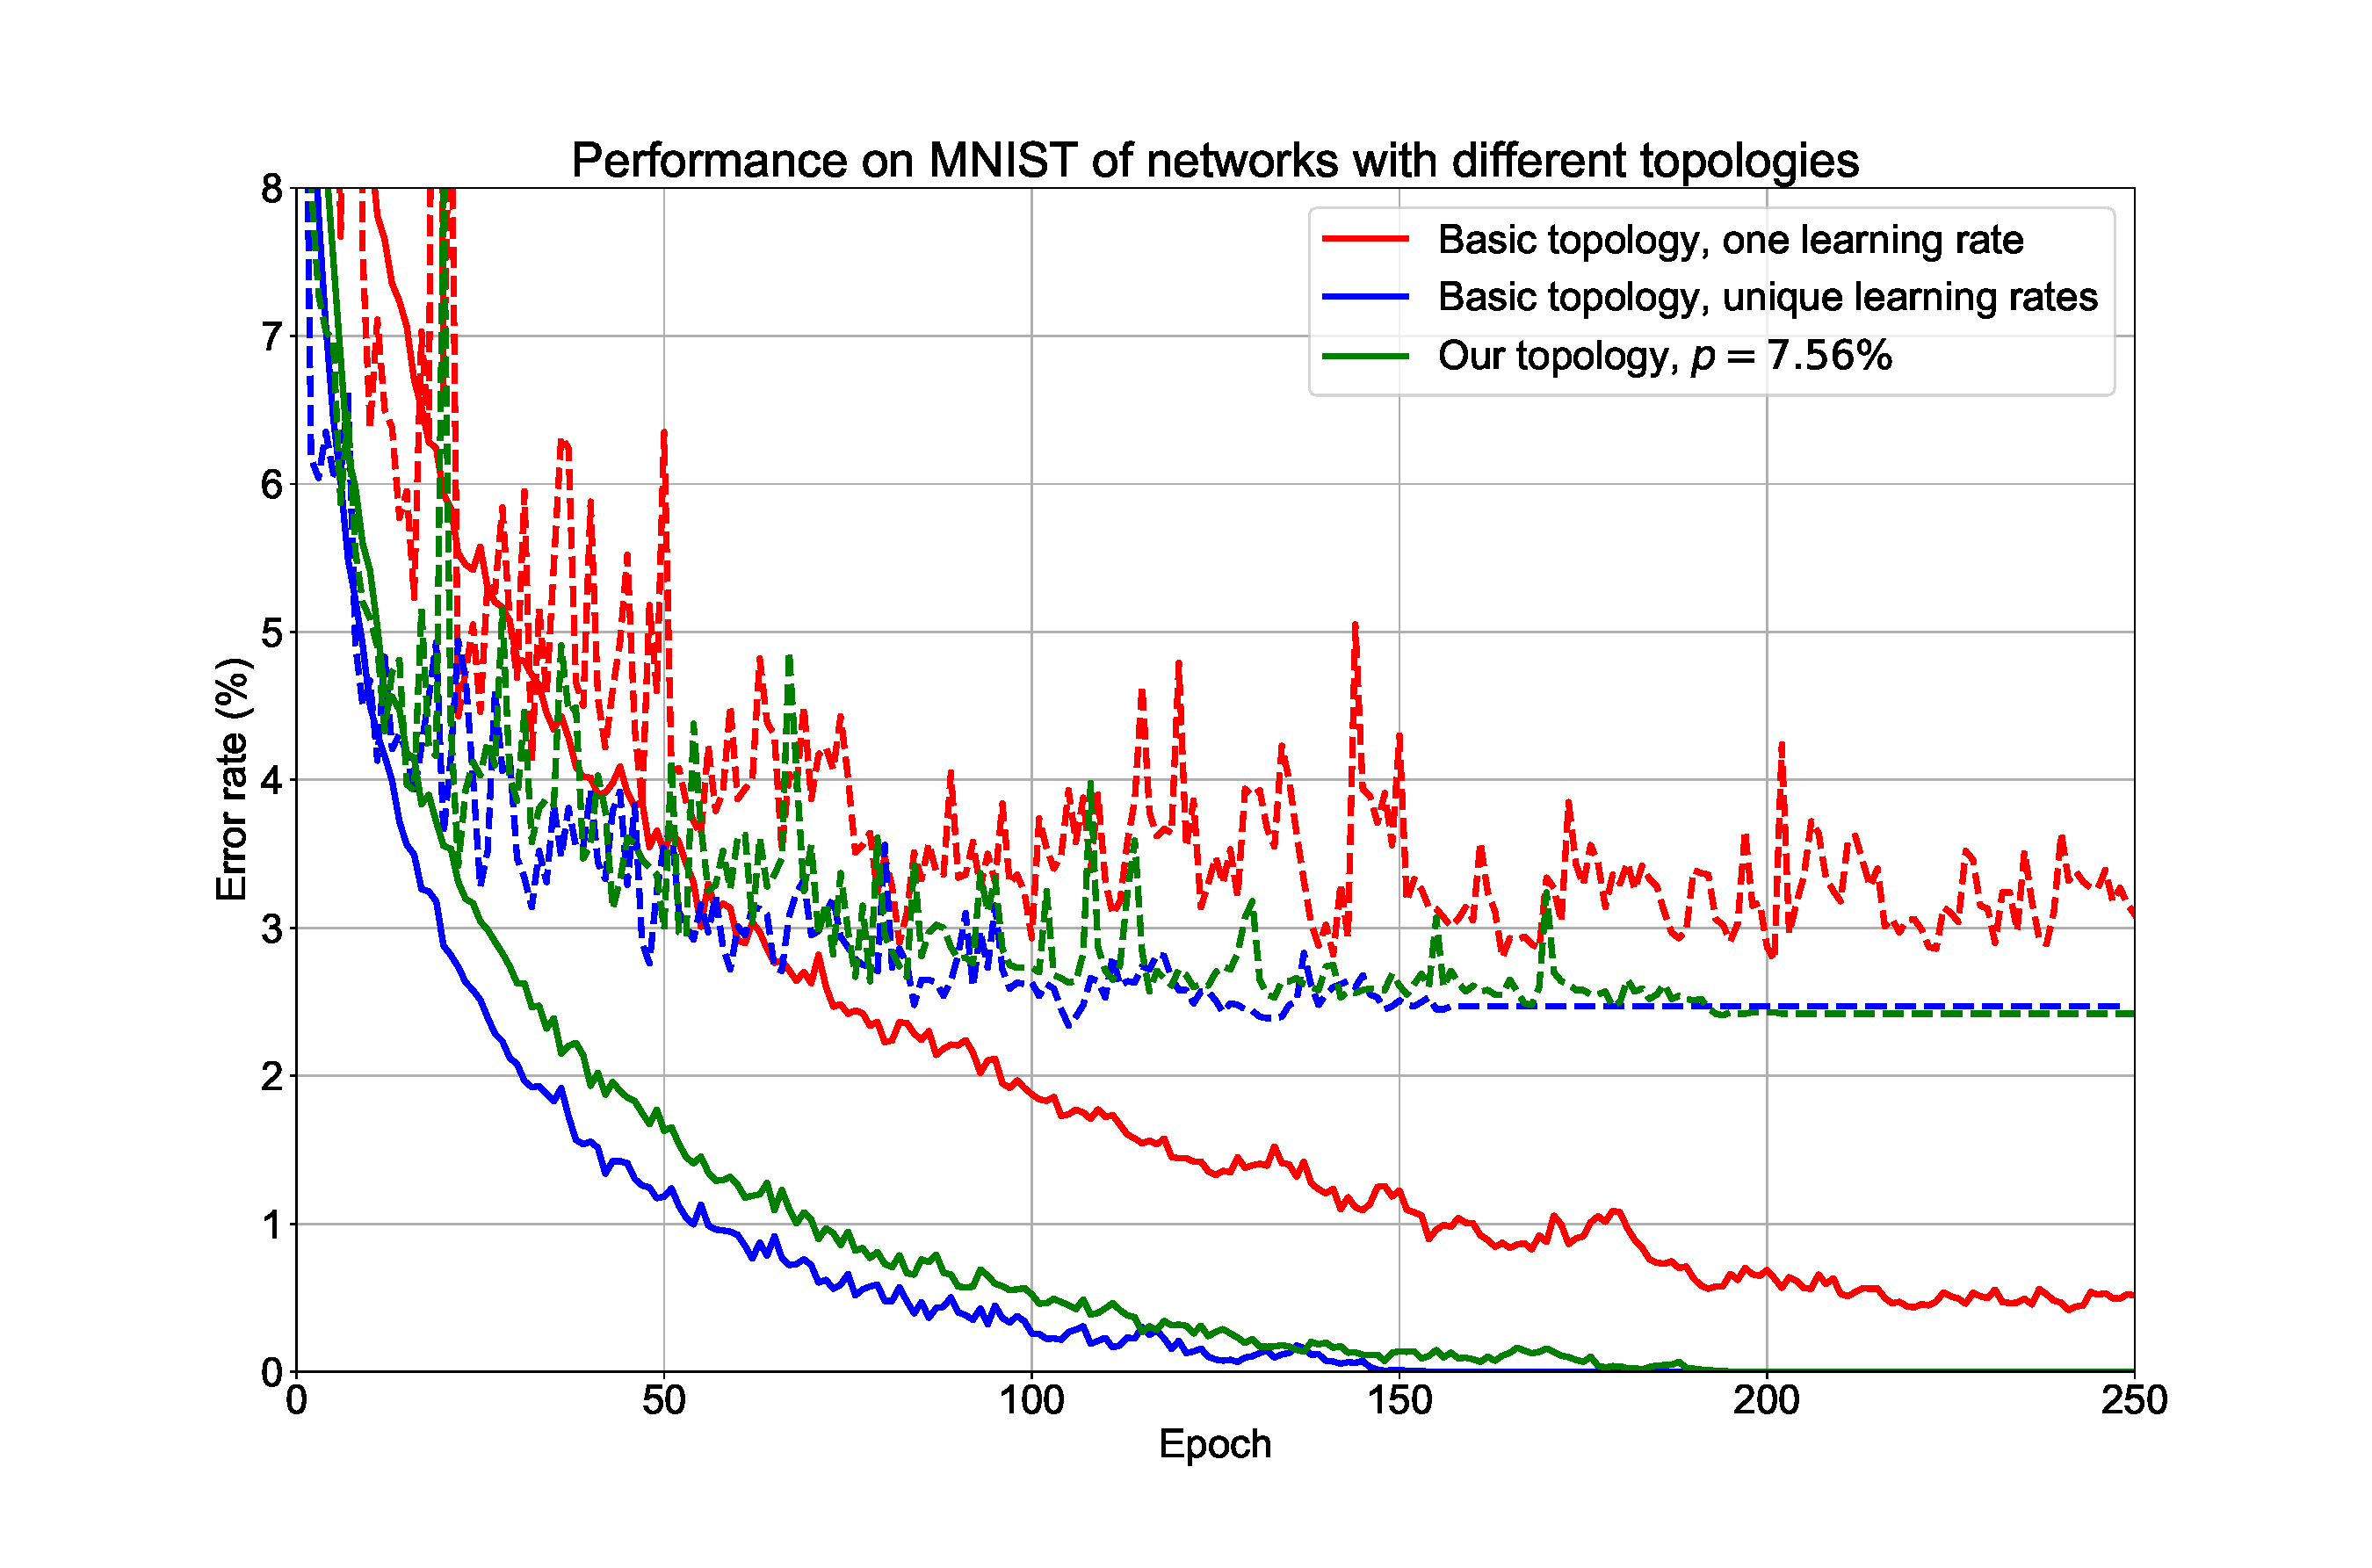
\includegraphics[width=\columnwidth]{figures/MNIST_network_comparison.pdf}
  \caption{Comparison of performance of network topologies on MNIST dataset. Dotted lines show test error and solid lines show training error. In red is a network with the basic topology and a single learning rate (section \ref{sec:basic_topology_uniform}). In blue is a network with the basic topology and unique learning rates (section \ref{sec:basic_topology}), tuned to counter the vanishing gradient problem; this is a recreation of the 5-layer network in \cite{scellier17}. In green is a network with our topology, $p=7.56\%$ (section \ref{sec:our_topology}). The network with a basic topology and a single learning rate performs poorly because it suffers from the vanishing gradient problem. The problem can be solved by introducing unique learning rates, or by implementing our topology.}
  \label{fig:mnist_comparison}
\end{figure}

\begin{table}
\begin{center}
\begin{tabular}{|c|c|c|c|c|c|c|c|c|}
\hline
Network topology & Learning rate(s) & $\epsilon$ & $\beta$ & $N_{free}$ & $N_{weakly-clamped}$\\\hline\hline
Basic, unique learning rates & .128, .032, .008, .002 & .5 & 1.0 & 500 & 8 \\\hline
Basic, one learning rate & .02 & .5 & 1.0 & 500 & 8  \\\hline
Our topology, $p=7.56\%$ & .02 & .5 & 1.0 & 500 & 8 \\\hline
\end{tabular}
\end{center}
\caption{Hyperparameters of networks tested on MNIST dataset}
\label{table:hyperparameters}
\end{table}

We compared the three network topologies described in sections \ref{sec:basic_topology}, \ref{sec:basic_topology_uniform}, and \ref{sec:our_topology} on the MNIST dataset \cite{mnist1998}. The hyperparameters for the networks are shown in table \ref{table:hyperparameters}. All networks were trained for 250 epochs with 50,000 training examples, 10,000 test examples and a batch size of 20.

\subsection{Network performance comparison}
\label{sec:network_performance}

We tracked the error rates of the three networks as they were trained and found that the network with our topology significantly outperforms the basic network with one learning rate, and achieves the same error rates as the basic network with unique learning rates in around 25\% more epochs. These results are shown in figure \ref{fig:mnist_comparison}.
\npar
 Notice that the basic network with unique learning rates converges to 0\% training error and 2.5\% test error in around 150 epochs and the network with our topology converges to 0\% training error and 2.5\% test error in around 190 epochs, whereas the basic network with one learning rate fails to converge in 250 epochs and has training and test error around .5\% higher than the other two networks. While it is possible that the basic network with one learning rate would converge given enough time, it is clearly inferior to the other two networks. It is also apparent that in the context of the MNIST dataset, our network with a single learning rate is practically interchangeable with the basic network with unique learning rates.

\subsection{Training rates of individual pairs of layers}
\label{sec:mnist_perlayer}

\begin{figure}
  \centering
  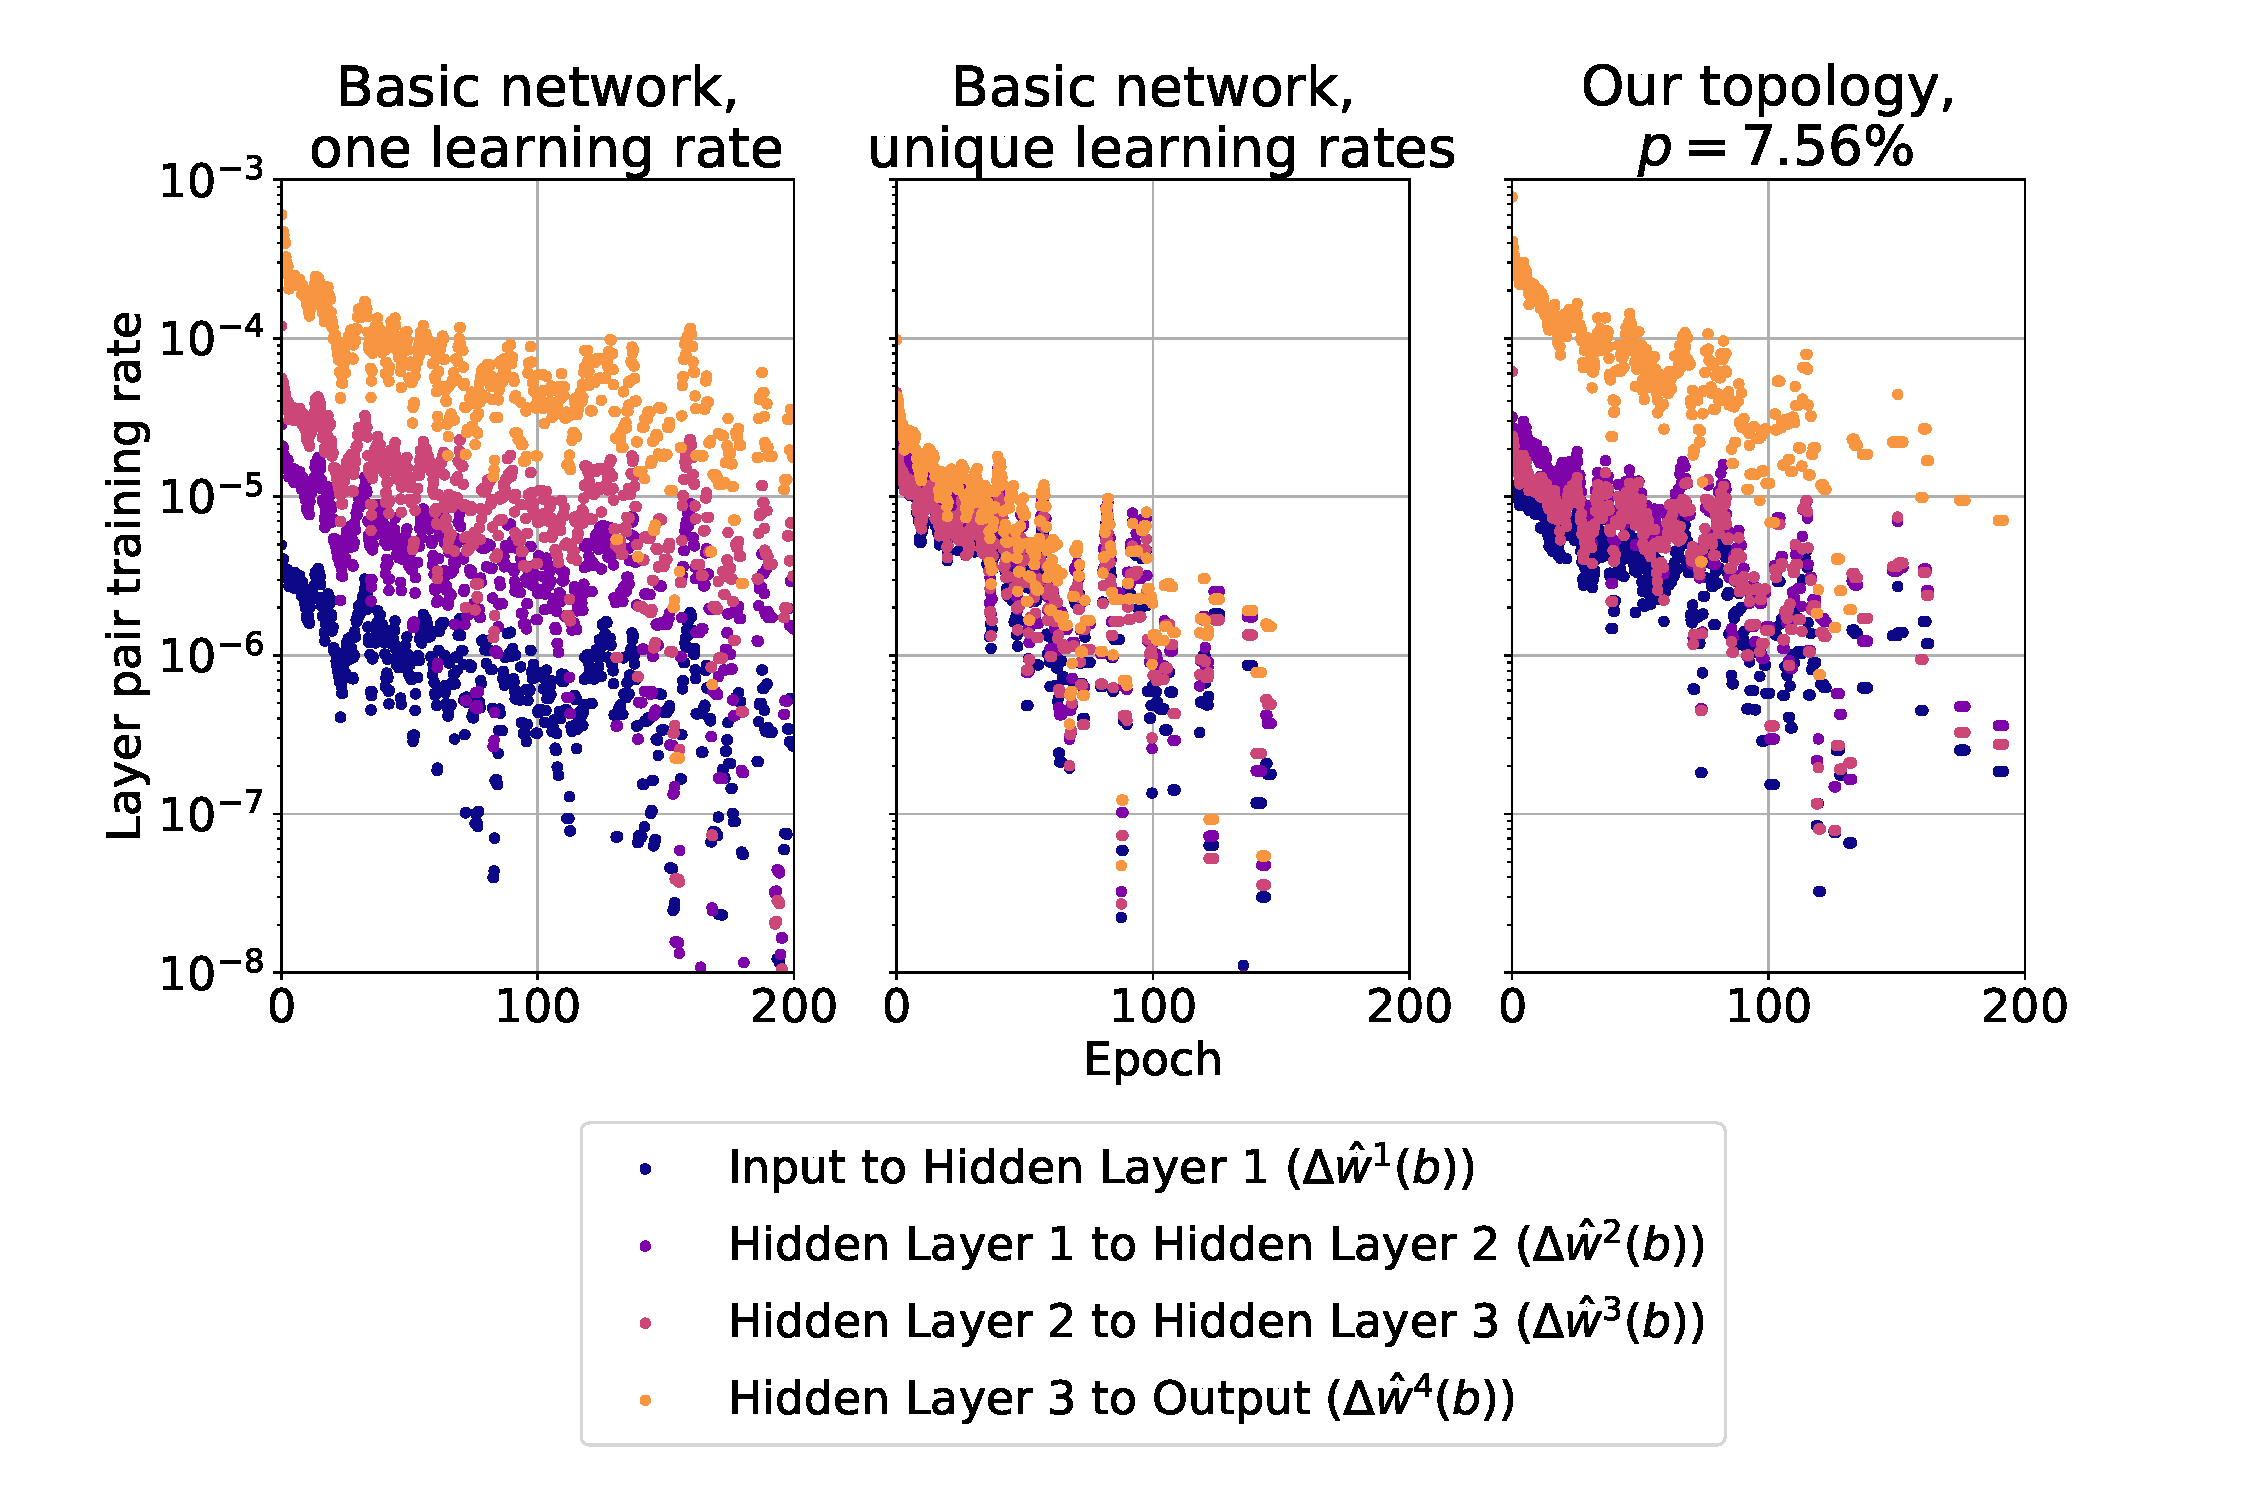
\includegraphics[width=\columnwidth]{figures/MNIST_individual_layers.pdf}
  \caption{Observation of extent of training of individual layers for different network topologies. Measurements were taken while running trials shown in figure \ref{fig:mnist_comparison}, and have been averaged as described in (\ref{eqn:layer_averaging}). To the left is a network with a standard multilayer feedforward topology and a single learning rate. In the center is a network with the same multilayer feedforward topology and unique learning rates for each layer, as described in \cite{scellier17}. To the right is a network with a multilayer feedforward topology with fully-connected layers and $p=7.56\%$.}
  \label{fig:mnist_layers}
\end{figure}

We tracked the training rates of individual pairs of layers as described in equations \ref{eqn:rms_correction} and \ref{eqn:running_avg} and found evidence that the extent of the vanishing gradient problem is the primary cause of the performance disparity seen in section \ref{sec:network_performance}. These results are shown in figure \ref{fig:mnist_layers}.
\npar
Notice in the basic network with one learning rate that there is a significant spread in the training rates of pairs of layers, with the deepest pair training at around 1\% of the rate of the shallowest pair. This problem is solved very effectively in the basic network with unique learning rates. The problem appears to be solved effectively for the deepest 3 pairs in the network with our topology, but the output layer still trains significantly faster than the deeper 3 layers. This makes sense if we assume that the important factor in a layer's training rate is its expected path length to the target layer, because every neuron in the output layer connects to the target layer through a single connection, whereas paths starting at deeper neurons must first pass through the output layer before connecting to the target layer.

\subsection{Error rate after one epoch as connections are added}
\label{sec:mnist_1epoch}

\begin{figure}
  \centering
  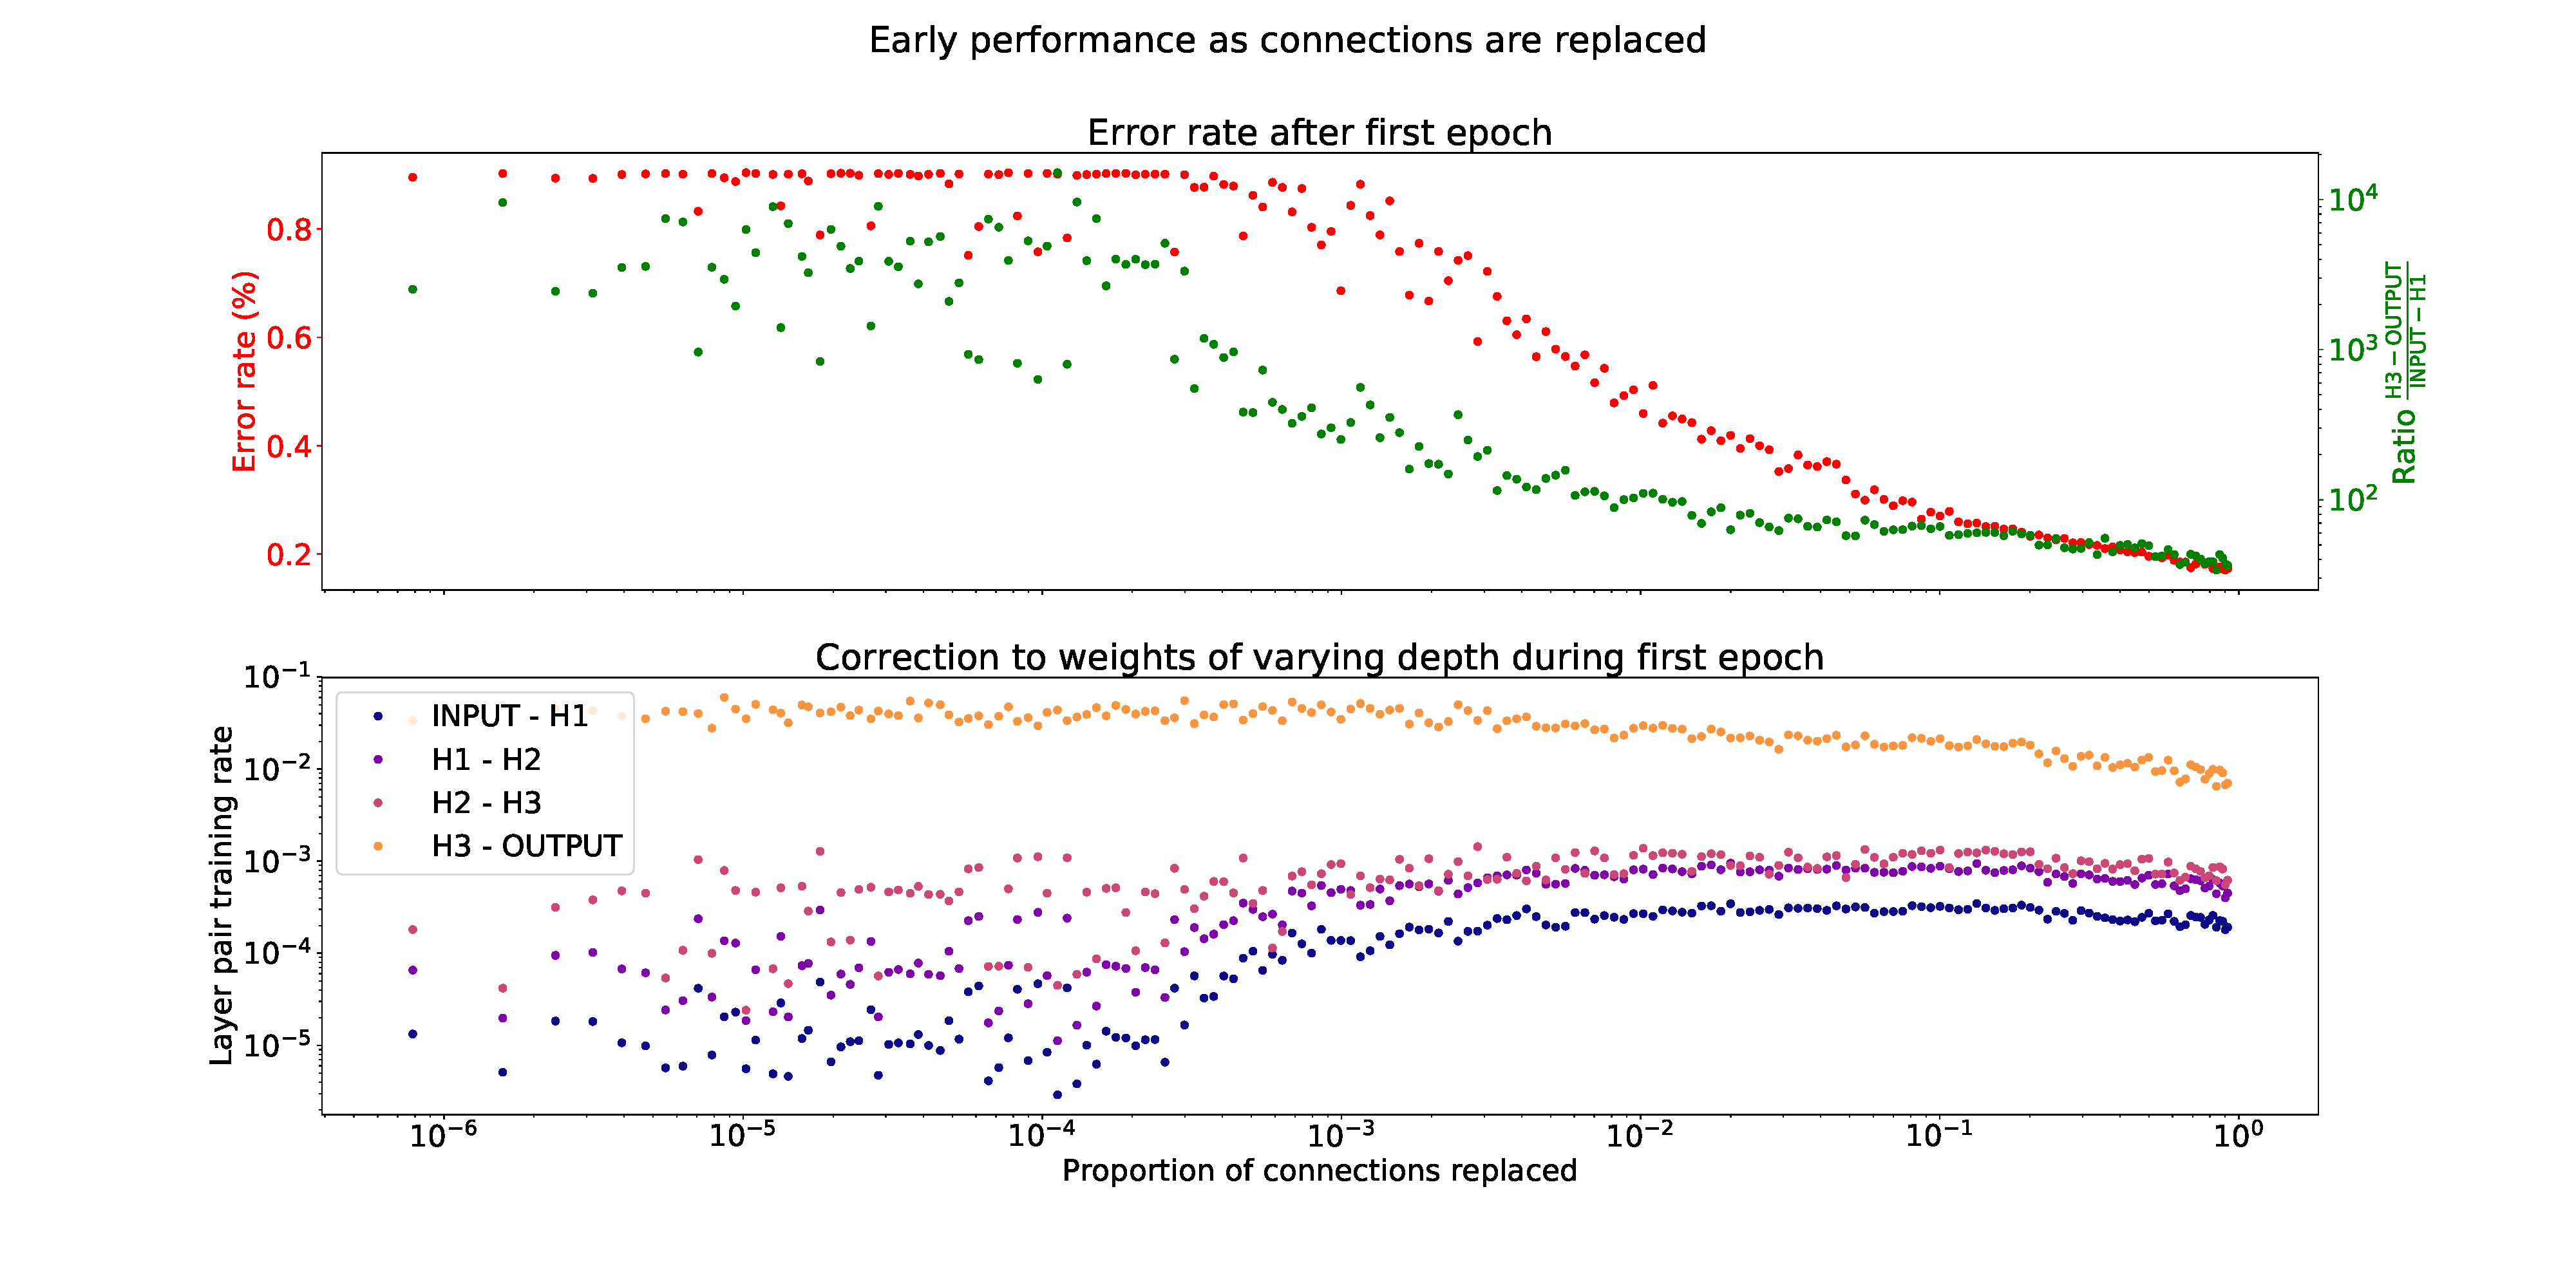
\includegraphics[width=\columnwidth]{figures/MNIST_one_epoch_performance.pdf}
  \caption{Performance of a network with our topology (section \ref{sec:our_topology}) with varying $p$. The top graph shows the training error after one epoch. The bottom graph shows the extent to which weights connecting each pair of layers was corrected over the epoch. It can be seen that there is little improvement for $p<10^{-4}$, rapid improvement for $10^{-4}<p<10^{-2}$ and little improvement for $p>10^{-2}$. The training error after one epoch decreases as pairs of layers train more uniformly with respect to depth.}
  \label{fig:mnist_1epoch}
\end{figure}

We tracked the training error after one epoch of a network with our topology, with varying numbers of layer-skipping connections and found that the error rate decays approximately exponentially. These results are shown in figure \ref{fig:mnist_1epoch}.
\npar
The error rate drops quickly as connections are replaced early on. We believe this is because when a forward connection is added, in addition to providing a path via. one connection between the two connected neurons, it also provides paths via. at most 3 jumps to all pairs of neurons in the two layers, as a result of the intralayer connectivity. This benefit is exhausted when all pairs of layers are connected, leading to the more-gradual improvement later on. It appears to take around 25,000 replaced connections to reach this regime, likely because the extent of attenuation of a gradient depends less on the minimum path length between two neurons and more on the number of low-attenuation paths it has available.
\npar
We found that our topology performs significantly worse than the basic topology with one learning rate when few connections are replaced, possibly due to inappropriate hyperparameter choices for intraconnected layers. We have seen some evidence that replacement of connections makes a network more-forgiving of poor weight matrix initialization, but have not thoroughly probed the issue.



\section{Conclusion}

We believe that our topology is a suitable substitute for unique learning rates as a solution to the vanishing gradient problem. While it is not as effective, it is simpler, more biologically-plausible, and would be easier to implement in an analog computer.
\npar
There are several directions in which future research could be taken. It would be useful to find and mathematically-justify an effective weight initialization scheme for a network with our topology. It would be interesting to explore the effect of adding (instead of replacing) layer-skipping connections, training a network, then removing the connections and training it further, to see if they provide a residual benefit even after removal; doing so could allow a network in an analog computer to be trained quickly, and the added connections removed to reduce the power consumption and heat load of the network. 


\bibliographystyle{plain}
%\nocite{*}
\bibliography{references}


\end{document}